\documentclass[12pt]{article}
\usepackage[utf8]{inputenc}
\usepackage[margin=.50in]{geometry}
\usepackage{textgreek}

    % Related to math
\usepackage{amsmath,amssymb,amsfonts,amsthm}
\usepackage{scrpage2}

\usepackage{tikz}

\pagestyle{scrheadings}

\title{Stochastik}
\author{Tassilo Tanneberger}
\newcommand{\linia}{\rule{\linewidth}{0.5pt}}
\makeatletter
\renewcommand{\maketitle}{\begin{center}
\huge \@title\end{center}
\linia\\
{\large\@author\hfill\@date\\}}

\begin{document}

\maketitle

\section{Wahrscheinlichkeit}

\paragraph{Notation} \( \neg A = A^C \) \newline \( \vert \Omega \vert = n \) Mächtigkeit \newline

\begin{tabular}{ |p{5cm}|p{12cm}|  }
 \hline
 \multicolumn{2}{|c|}{Zusammenfassung von Wahrscheinlichkeiten} \\
 \hline
Event & Wahrscheinlichkeit\\
 \hline
 A & \( P(A) \in [0, 1] \) \\
 not A & \( P(\neg A) = 1 - P(A) \) \\
 A oder B & \( P(A \cup B) = P(A) + P(B) - P(A \cap B) \)  \\
  & \(  P(A \cup B) = P(A) + P(B) \) Wenn A und B exclusiv sind \\
 A und B & \( P(A \cap B) = P(A\vert B)P(B) = P(B\vert A)P(A)\) \\
 & \( P(A \cap B) = P(A) \cdot P(B) \) Wenn A und B unabhängig sind\\
  A given B & \( P(A \vert B) = \frac{P(A \cap B)}{P(B)}\) \\
 \hline
\end{tabular}

\section{ Axiomsystem von Kolmogorow}

\begin{enumerate}
	\item Jedes Ereignis A \( P(A) \in [0,1] \land P(A) \in \mathbb{R} \vert A \in \Sigma \) 
	\item Sicheres Ereignis \( \Omega \in \Sigma \land P(\Omega) = 1 \)
	\item Wahrscheinlichkeits Vereinigung \( \bigcup_{i=1}^{n} (A_i) = \sum_{i=1}^n (A_i)\) siehe \( \sigma \) - additivät
	
\end{enumerate}

\section{ Laplace Experiment }

Endlich viele Elementarereignisse (\( E_i \)) wobei alle gleichberechtigt sind: 
\begin{align*}
P = \frac{1}{\vert \Omega \vert } \Rightarrow \Omega = \bigcup_{i=1}^{n} (E_i)
\end{align*}


Wenn Ereignisse (\( A \)) sich aus Elementarereignissen zusammen setzten Ist die Mächtigkeit dieses Ereigniss die anzahl der verknüpften Elementarereignisse \( \vert A \vert = m \).

\begin{align*}
P(A) = \frac{\vert A \vert }{\vert \Omega \vert }
\end{align*}


\newpage

\section{Bedingte Wahrscheinlichkeiten}
\begin{figure}[h]
	\center
	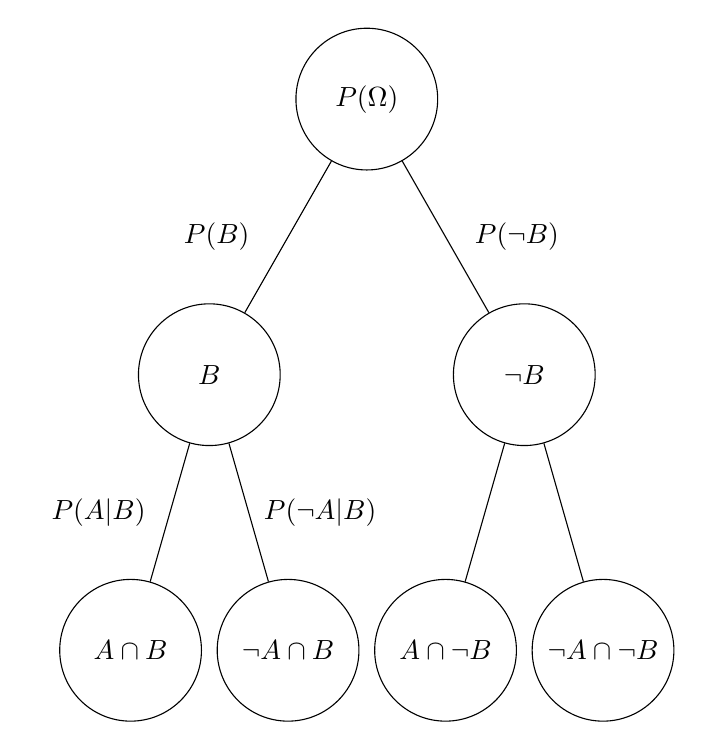
\begin{tikzpicture}[nodes={draw, circle}, 
	minimum size=1.8cm,
	sibling distance=3cm,
	level distance=3.5cm,
  	level 1/.style={sibling distance=4cm},
  	level 2/.style={sibling distance=2cm}]
  \node { $ P( \Omega )$ }
    child {node { $  B  $}
      child {node { $ A \cap B $}  edge from parent node [left,draw=none]{ $ P( A \vert B ) $} }
      child {node { $ \neg A \cap B$}  edge from parent node [right,draw=none]{ $ P( \neg A \vert B ) $}}
      edge from parent node [left,draw=none]{ $ P( B ) $}
    }
    child {node {  $ \neg B $}
    child {node {$ A \cap \neg B$}}
    child {node {$ \neg A \cap \neg B $}}
    edge from parent node [right,draw=none]{ $ P( \neg B ) $}
    };
\end{tikzpicture}
\end{figure}

Wenn sich die Wahrscheinlichkeit von A abhängig von dem dafor stattgefunden Event ist. Somit B die Wahrscheinlichkeit von A beinflusst.

\section{ Verbundswahrscheinlichkeiten }

\paragraph{Verknüpfen zweier Abhängiger Ereignisse}
\begin{align*}
P ( B \cap A) = P(A) \cdot P(B \vert A) = P(B) \cdot P( A\vert B)
\end{align*}

\paragraph{ Satz von Bayes}
\begin{align*}
	P( A \vert B ) = \frac{P(B \vert A) \cdot P(A)}{P(B)}
\end{align*}


\section{ Wahrscheinlichkeitsraum }

Wahrscheinlichkeitsraum \( ( \Omega, \Sigma, P) \) wobei P ein Wahrscheinlichkeitsmaß (siehe Axiome Kolgomorow) ist.

\begin{itemize}
	\item \( \Omega \neq \emptyset \) Ergebnismenge 
	\item \( \Sigma \) \( \sigma \) - Algebra über \( \Omega \Rightarrow \Sigma = \lbrace \lbrace E_1, \dots, E_n \rbrace \vert \forall i \in [1, \dots, n] : E_i = \lbrace x_1, \dots, x_m \vert x_j \in \Omega, j \in [1, \dots,m \rbrace \rbrace \rbrace \) Ereignissystem
	\item \( P:\Sigma \rightarrow [0, 1] \) Wahrscheinlichkeitsmaß - Ordnet Ereignissen ihre Wahrscheinlichkeit zu.
\end{itemize}

\section{ Kenngrößen }

\subsection*{Erwartungswert }

\begin{align*}
	\mu = \sum_{i=1}^{n} x_i \cdot  P(X=x_i) \mid n \in \mathbb{N}
\end{align*}
	 
\subsection*{Varianz / Streuung / Dispersion}

\begin{align*}
	Var(X) := \mathbb{E}((X-\mu)^2) = \int_{\Omega}^{} (X-\mu)^2 dP = \sum_{i=1}^{n} (x_i - \mu)^2 \cdot  P(X=x_i)
\end{align*}	 
	 
\subsection*{Standart Abweichung }

\begin{align*}
	\sigma = \sqrt{Var(X)} = \sqrt{\sum_{i=1}^{n} (x_i - \mu)^2 \cdot  P(X=x_i)} \mid n \in \mathbb{N} 
\end{align*}



\section{ Kombinatorik }
\subsection*{ Permutation }

Ohne Wiederholung: \( P_n = n! \) \newline
Mit Wiederholung: \( P_n ^{k} = \frac{n!}{\Sigma k_i} \)

\subsection*{Variation}

Ohne Wiederholung: \( V_n^k = \frac{n!}{(n-k)!} \) \newline
Mit Wiederholung: \( V_n^k = n^k \) \newline

\subsection*{Kombination}

Ohne Wiederholung: \( K_n^k = \begin{pmatrix}
n \\ k 
\end{pmatrix} = \frac{n!}{k! \cdot (n-k)!} \) \newline
mit Wiederholung: \( K_n^k = \begin{pmatrix}
n + k - 1\\ k 
\end{pmatrix} \)

\section{Wahrscheinlichkeits Verteilungen}

\subsection*{ Bernoulli - Prozesse }

Ist ein dirkreter stochastischer Prozess der endlich viele unabhänige Versuche mit Bernoulli - Verteilung also \( p \in [0, 1] \)

\subsection*{ Binomialverteilung }

\begin{align*}
	B(k \vert p, n) = 
	\begin{cases}
    \begin{pmatrix}
	n \\ k 
	\end{pmatrix} \cdot p^k \cdot (1 - p)^{n-k},& \text{if } k \in \lbrace 0, \dots, n \rbrace \\
    0,              & \text{otherwise}
	\end{cases}	
\end{align*}
\( p \dots \text{Eintritts Wahrscheinlichkeit } \) \newline
\( n \dots \text{Anzahl durchgeführter Versuche} \) \newline
\( k \dots \text{Gewünschte Anzahl positiver resultate}\)

\paragraph{ Intuition Entwicklung }

\( p^k \cdot (1 - p)^{n-k} \) Ist die Wahrscheinlichkeit des eintretens 
\( \begin{pmatrix}
	n \\ k 
\end{pmatrix} \) Und da die Reinfolge keine Rolle spielt ist die Wahrscheinlichkeit mit den Anordnungsmöglichkeiten zu Multiplizieren. \newline

\paragraph{Kenngrößen}
\begin{itemize}
	\item Erwartungswert: \( \mu = np \)
	\item Varianz: \( Var(X) = np(1-p)  \)
	\item Standard Abweichung: \( \sigma(X) = \sqrt{np(1-p)}  \)
\end{itemize}

\paragraph{kumulierte Binomialverteilung}
\begin{align*}
	F(n,p,k) = P(X \leq k) = \sum_{i=0}^{i} \begin{pmatrix}
	n \\ i 
	\end{pmatrix} \cdot p^k \cdot (1 - p)^{n-i}
\end{align*}


\end{document}